%-------------------------
% Resume in Latex
% Author : Jake Gutierrez
% Based off of: https://github.com/sb2nov/resume
% License : MIT
%------------------------

\documentclass[letterpaper,11pt]{article}

\usepackage{latexsym}
\usepackage[empty]{fullpage}
\usepackage{titlesec}
\usepackage{marvosym}
\usepackage[usenames,dvipsnames]{color}
\usepackage{xcolor}
\usepackage{verbatim}
\usepackage{enumitem}
\usepackage[hidelinks]{hyperref}
\usepackage{fancyhdr}
\usepackage[english]{babel}
\usepackage{tabularx}
\usepackage{fontawesome}
\usepackage{ifthen} % For conditional statements
\usepackage{tikz}
\usepackage{array}
\usepackage{colortbl} % Required for \arrayrulecolor
\usepackage{changepage}
\usepackage{fancyhdr}
\usepackage{lastpage}
\usepackage{datetime}
\input{glyphtounicode}

\usepackage[
  sorting=ydnt, % Sorts entries by year (descending order), name, title
	style=authoryear,
	doi=false,
	isbn=true,
	url=false,
	eprint=false,
	backref = false, % include back references in bibliography
	maxcitenames=3, % affects only the citations in the document body
	maxbibnames=99, % affects only the bibliography, pass 99 to print all
	hyperref=true,
	block=none,
	backend=biber % {Options: bibtex, biber}
	]{biblatex}
\addbibresource{bib.bib}



%----------FONT OPTIONS----------
% sans-serif
% \usepackage[sfdefault]{FiraSans}
\usepackage[sfdefault]{roboto}
\usepackage[T1]{fontenc} % to use \l (The polish l)
% \usepackage[sfdefault]{noto-sans}
% \usepackage[default]{sourcesanspro}

% serif
% \usepackage{CormorantGaramond}
% \usepackage{charter}

% Define a toggle for including the photo
\newboolean{includephoto}

\pagestyle{fancy}
\fancyhf{} % Clear all header and footer fields

\renewcommand{\today}{\number\day~\ifcase\month\or January\or February\or March\or April\or May\or June\or July\or August\or September\or October\or November\or December\fi, \number\year}
% Define footer
\fancyfoot[C]{\color{gray}\sffamily \makebox[.9\paperwidth]{\hfill Resume \textbullet\ \today \hfill \thepage/\pageref{LastPage}}}
\setlength{\footskip}{15pt} % Increase this value to lower the footer

\renewcommand{\headrulewidth}{0pt}
\renewcommand{\footrulewidth}{0pt}

% Adjust margins
\addtolength{\oddsidemargin}{-0.5in}
\addtolength{\evensidemargin}{-0.5in}
\addtolength{\textwidth}{1in}
\addtolength{\topmargin}{-.5in}
\addtolength{\textheight}{1.0in}

\urlstyle{same}

\raggedbottom
\raggedright
\setlength{\tabcolsep}{0in}

% Sections formatting
\titleformat{\section}{
  \vspace{-4pt}\scshape\raggedright\large\color{alt}
}{}{0em}{}[\color{alt}\titlerule \vspace{-5pt}]

% Ensure that generate pdf is machine readable/ATS parsable
\pdfgentounicode=1

\definecolor{graytext}{HTML}{666666}
\definecolor{alt}{HTML}{000f7e}
\setboolean{includephoto}{false} % Set to true to include the photo, false otherwise

%~~~~~~~~~~~~~~~~~~~~~~~~~~~~~~~~~~~~~~~~~~~~~~~~~~~~~~~~~~~~~~~~~~~~~~~~~~~~~~~~
%~~~~~~~~~~~~~~~~~~~~~~~~~~~~~CV RELATED~~~~~~~~~~~~~~~~~~~~~~~~~~~~~~~~~~~~~~~~~
%~~~~~~~~~~~~~~~~~~~~~~~~~~~~~~~~~~~~~~~~~~~~~~~~~~~~~~~~~~~~~~~~~~~~~~~~~~~~~~~~
\newcommand{\resumeItem}[1]{
  \item\small{
    {#1 \vspace{-2pt}}
  }
}

\newcommand{\resumeSubheadingUnbold}[4]{
    \vspace{-2pt}\item
    \hspace*{-.0cm}\begin{tabular*}{0.97\textwidth}[t]{ll@{\extracolsep{\fill}}r}
      \textbullet & \hspace*{-.6cm}#1                & #2 \\
                  & \hspace*{-.6cm}\textit{\small#3} & \textit{\small #4} \\
    \end{tabular*}\vspace{-7pt}
}

\newcommand{\resumeSubheading}[4]{
  \vspace{-2pt}\item
    \begin{tabular*}{0.97\textwidth}[t]{l@{\extracolsep{\fill}}r}
      \textbf{#1} & #2 \\
      \textit{\small#3} & \textit{\small #4} \\
    \end{tabular*}\vspace{-7pt}
}

\newcommand{\resumeSubSubheading}[2]{
    \item
    \begin{tabular*}{0.97\textwidth}{l@{\extracolsep{\fill}}r}
      \textit{\small#1} & \textit{\small #2} \\
    \end{tabular*}\vspace{-7pt}
}

\newcommand{\resumeProjectHeading}[2]{
    \item
    \begin{tabular*}{0.97\textwidth}{l@{\extracolsep{\fill}}r}
      \small#1 & #2 \\
    \end{tabular*}\vspace{-7pt}
}

\newcommand{\resumeSubItem}[1]{\resumeItem{#1}\vspace{-4pt}}

\renewcommand\labelitemii{$\vcenter{\hbox{\tiny$\bullet$}}$}

\newcommand{\resumeSubHeadingListStart}{\begin{itemize}[leftmargin=0.15in, label={}]}
\newcommand{\resumeSubHeadingListEnd}{\end{itemize}}
\newcommand{\resumeItemListStart}{\begin{itemize}}
\newcommand{\resumeItemListEnd}{\end{itemize}\vspace{-5pt}}

%~~~~~~~~~~~~~~~~~~~~~~~~~~~~~~~~~~~~~~~~~~~~~~~~~~~~~~~~~~~~~~~~~~~~~~~~~~~~~~~~
%~~~~~~~~~~~~~~~~~~~~~~~~~~~~~~~~~~~~~~~~~~~~~~~~~~~~~~~~~~~~~~~~~~~~~~~~~~~~~~~~


%~~~~~~~~~~~~~~~~~~~~~~~~~~~~~~~~~~~~~~~~~~~~~~~~~~~~~~~~~~~~~~~~~~~~~~~~~~~~~~~~
%~~~~~~~~~~~~~~~~~~~~~~~~~~~BIBLIOGRAPHY~~~~~~~~~~~~~~~~~~~~~~~~~~~~~~~~~~~~~~~~~
%~~~~~~~~~~~~~~~~~~~~~~~~~~~~~~~~~~~~~~~~~~~~~~~~~~~~~~~~~~~~~~~~~~~~~~~~~~~~~~~~

% Avoid splitting entries across page break (only for 3 or fewer lines)
% Tip: http://tex.stackexchange.com/a/51261
\AtBeginEnvironment{thebibliography}{%
   \clubpenalty10000
   \@clubpenalty \clubpenalty
   \widowpenalty10000
   \interlinepenalty5000}

% Customized format, based on the Fancy CV template created by Adrien Friggeri
% See https://github.com/ashee/cv (MIT license)
\DeclareFieldFormat[article]{title}{#1\par}
\DeclareFieldFormat[inproceedings]{title}{#1\par}
\DeclareFieldFormat[misc]{title}{#1\par}
\DeclareFieldFormat[report]{title}{#1\par}
\DeclareFieldFormat[incollection]{title}{#1\par}

\DeclareBibliographyDriver{article}{%
  \small
  \textbf{\printfield{year}}\hspace{.2cm} % 
  \printfield{title}%
  \newblock%
  \hspace{.51cm}\printnames{author}%
  \par%
  \newblock%
  \hspace{.45cm} {%
    \small\color{graytext}
    \usebibmacro{journal+issuetitle}%
    \setunit{\space}%
    \printfield{pages}%
    \newunit%
    \printlist{publisher}%
    \setunit*{\addcomma\space}%
    \newunit%
  }
  \par\vspace{0.3\baselineskip}
}

\DeclareBibliographyDriver{inproceedings}{%
  \small
  \printfield{title}%
  \newblock%
  \printnames{author}%
  \par%
  \newblock%
  {%
    \small\color{graytext}%
    \printfield{booktitle}%
    \setunit{\addcomma\space}%
    \printfield{year}%
    \setunit{\addcomma\space}%
    \printlist{location}%
    \newunit%
  }
  \par\vspace{0.3\baselineskip}
}

\DeclareBibliographyDriver{incollection}{%
  \small
  \printfield{title}%
  \newblock%
  \printnames{author}%
  \par%
  \newblock%
  {%
    \small\color{graytext}%
    \printfield{booktitle}%
    \setunit{\addcomma\space}%
    \printfield{year}%
    \setunit{\addcomma\space}%
    \printlist{location}%
    \newunit%
  }
  \par\vspace{0.3\baselineskip}
}

\DeclareBibliographyDriver{misc}{%
  \small
  \printfield{title}%
  \newblock%
  \printnames{author}%
  \par%
  \newblock%
  {%
    \small\color{graytext}%
    \printfield{booktitle}%
    \setunit*{\addcomma\space}%
    \printfield{note}%
    \setunit*{\addcomma\space}%
    \printfield{year}%
    \setunit{\addcomma\space}%
    \printlist{location}%
    \newunit%
  }
  \par\vspace{0.3\baselineskip}
}

\DeclareBibliographyDriver{report}{%
  \small
  \printfield{title}%
  \newblock%
  \printnames{author}%
  \par%
  \newblock%
  {%
    \fontsize{8pt}{1em}\bodyfontlight\color{graytext}%
    \printfield{type}%
    \setunit{\space}%
    \printfield{number}%
    \setunit{\addcomma\space}%
    \printfield{year}%
    \newunit%
  }
  \par\vspace{0.3\baselineskip}
}


% New syntax for flexible backend (BibLaTeX > v3.3)
\DeclareNameFormat{author}{%
  \small
  \renewcommand*{\multinamedelim}{\addcomma\addspace}%
  \nameparts{#1}%
  \ifthenelse{\value{listcount}=1}
    {\expandafter\ifstrequal\expandafter{\namepartfamily}{Monaco}{\textbf{\namepartgiven\space\namepartfamily}}{\namepartgiven\space\namepartfamily}}%
    {\expandafter\ifstrequal\expandafter{\namepartfamily}{Monaco}{\textbf{\namepartgiven\space\namepartfamily}}{\namepartgiven\space\namepartfamily}}%
  \ifthenelse{\value{listcount}<\value{liststop}}
  {\addcomma\space}
  {}
}
%-------------------------------------------
%%%%%%  RESUME STARTS HERE  %%%%%%%%%%%%%%%%%%%%%%%%%%%%
\begin{document}
%----------HEADING----------
% \begin{tabular*}{\textwidth}{l@{\extracolsep{\fill}}r}
%   \textbf{\href{http://sourabhbajaj.com/}{\Large Sourabh Bajaj}} & Email : \href{mailto:sourabh@sourabhbajaj.com}{sourabh@sourabhbajaj.com}\\
%   \href{http://sourabhbajaj.com/}{http://www.sourabhbajaj.com} & Mobile : +1-123-456-7890 \\
% \end{tabular*}


\ifthenelse{\boolean{includephoto}}{
  \def\posx{0}
  \def\posy{0}
  \def\imgsize{1.7cm}
  \vspace*{-1cm}
  \begin{minipage}{.5cm}
    ~
  \end{minipage}
  \begin{minipage}{4cm}
    \begin{tikzpicture}
      % Define the circular clipping path
      \clip (\posx, \posy) circle (\imgsize);
      % Place the image inside the clipping path
      \node[anchor=center] at (\posx, \posy) {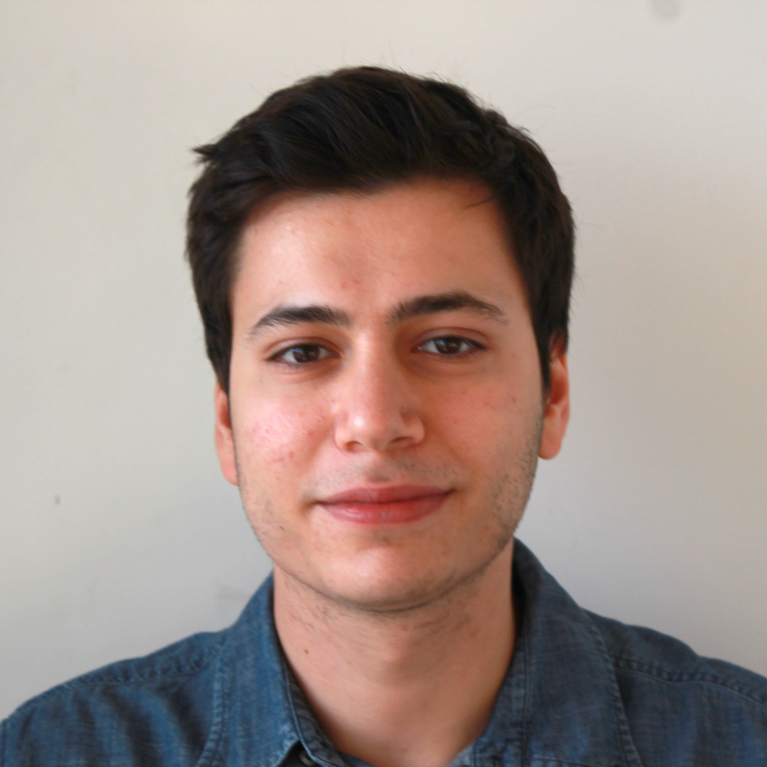
\includegraphics[width=3.5cm]{../../images/profile.png}};
      % Add a circular border around the clipped image
      \draw[alt, line width=2mm] (\posx, \posy) circle (\imgsize) {};
    \end{tikzpicture}
  \end{minipage}
  \begin{minipage}{.6\linewidth}
      {\Huge \scshape Saverio \textbf{Monaco}} \\[3pt] 
      {\color{alt}Computational Physicist \,\textbullet\, Machine Learning Researcher}\\[2pt]
      \small \href{mailto:saverio.monaco@desy.de}{
        {\color{alt}\faEnvelope~} \underline{saverio.monaco@desy.de}} $|$~ 
      \href{https://linkedin.com/in/saverio-monaco}{
        {\color{alt}\faLinkedinSquare~} \underline{linkedin.com/in/saverio-monaco}} $|$~\\
      \href{https://github.com/SaverioMonaco}{
        {\color{alt}\faGithub~} \underline{github.com/SaverioMonaco}}
  \end{minipage}
}{
  \begin{center}
      {\Huge \scshape Saverio \textbf{Monaco}} \\ \vspace{5pt}
      \small \href{mailto:saverio.monaco@desy.de}{
        {\color{alt}\faEnvelope~} \underline{saverio.monaco@desy.de}} $|$~ 
      \href{https://linkedin.com/in/saverio-monaco}{
        {\color{alt}\faLinkedinSquare~} \underline{linkedin.com/in/saverio-monaco}} $|$~
      \href{https://github.com/SaverioMonaco}{
        {\color{alt}\faGithub~} \underline{github.com/SaverioMonaco}}
  \end{center}
}

%-----------EDUCATION-----------
\section{Education}
  \resumeSubHeadingListStart
    \resumeSubheading
      {RWTH Aachen University \& DESY}{Hamburg, Germany}
      {PhD in Quantum Generative models for High Energy Physics - ENGAGE}{Mar. 2024 -- Present}
      {
        ~\\
        \textit{\small{Marie Sk{\l}odowska-Curie PhD}}\\
        \textit{\quad \small\textbullet~ \textbf{Thesis}: Detector Simulation and Jet Clustering for HL LHC with Quantum Computing}
      }
    \resumeSubheading
      {University of Padua}{Padua, Italy}
      {M.Sc. in Computational Physics}{Sep. 2020 -- Sep. 2023}
      {
        ~\\
        \textit{\quad \small\textbullet~ \textbf{Thesis}: Study of Quantum Correlations in LHCb simulated heavy flavour jets}\\
        \textit{\quad \small\textbullet~ \textbf{Honors}: Magna cum laude}
      }
    \resumeSubheading
      {University of Catania}{Catania, Italy}
      {B.Sc. in Physics}{Sep. 2016 -- Jul. 2020}
      {
        ~\\
        \textit{\quad \small\textbullet~ \textbf{Thesis}: Phase‑Space Formulation of Quantum Mechanics}
      }
  \resumeSubHeadingListEnd


%-----------EXPERIENCE-----------
\section{Experience}
  \resumeSubHeadingListStart
    \resumeSubheading
      {Quantum Machine Learning Intern}{Geneva, Switzerland}
      {CERN}{Apr. 2022 -- Aug. 2022}
      \resumeItemListStart
        \resumeItem{Explored Quantum Machine Learning techniques for phase detection in the ANNNI spin model.}
        \resumeItem{Developed and implemented supervised and unsupervised architectures for phase detection.}
        \resumeItem{Published a Python package under the CERN-IT organization.}
        \resumeItem{Authored and published a paper on the implemented techniques.}
      \resumeItemListEnd

  \resumeSubHeadingListEnd

%
%-----------PROGRAMMING SKILLS-----------
\section{Technical Skills}
 \begin{itemize}[leftmargin=0.15in, label={}]
    \small{\item{
     \textbf{Quantum Computing tools}{: Pennylane, Qiskit, Quimb, YAOML.jl}\\
     \textbf{Programming languages}{: Python, Julia, C/C++, SQL, R, VHDL, Agda, TeX, Nix} \\
     \textbf{Machine Learning libraries}{: Jax, Pytorch, Keras}\\
     \textbf{Other libraries}{: Pandas, NumPy, Matplotlib, BeautifulSoup}\\
     \textbf{Other Tools}{: Git, Docker, Vim, Linux, Sphinx, ReadTheDocs} \\
    }}
 \end{itemize}

%
%----------- LANGUAGES -----------
\section{Languages Spoken}
\textbf{Mother tongue:} Italian\\
\textbf{Other languages:}\\
\setlength{\tabcolsep}{12pt} % Adjust column spacing
\hspace*{1cm}
\begin{tabular}{ll|l|l|l}
  \arrayrulecolor{alt} % Set line color to alt
                   & \textcolor{alt}{Understanding} & \textcolor{alt}{Speaking} & \textcolor{alt}{Writing} & \textcolor{alt}{Certificate} \\
  \arrayrulecolor{black} % Set line color to black
  \textbf{English} & C1                             & C1                        & C1                       & IELTS Academic: score 7      \\
  \textbf{German}  & C1                             & B2                        & B2                       & Goethe-Zertifikat: B2        \\
  \textbf{French}  & B2                             & B1                        & B2                       & EsaBac Diploma               \\
  
\end{tabular}
%---------------------------------

%
%-----------PRESENTATIONS-----------
\section{Presentations}
  \resumeSubHeadingListStart
    \resumeSubheadingUnbold
      {\textbf{Poster presentation} @ QT4HEP 2025 (CERN)}{Geneve, Switzerland}
      {\textcolor{darkgray}{\textit{"Precise Quantum Angle Generator Designed for Noisy Quantum Devices"}}}{Jan. 2025}
    \resumeSubheadingUnbold
      {\textbf{Talk} @ The Helmholtz "Matter and the Universe" Days 2024 (DESY)}{Hamburg, Germany}
      {\textcolor{darkgray}{\textit{"Quantum Group @ DESY: Quantum Machine Learning for Calorimeter Simulation"}}}{Dec. 2024}
    \resumeSubheadingUnbold
      {\textbf{Poster presentation} @ QTech 2024 (Freie Universität Berlin)}{Berlin, Germany}
      {\textcolor{darkgray}{"Precise Quantum Angle Generator Designed for Noisy Quantum Devices"}}{Sep. 2024}
    \resumeSubheadingUnbold
      {\textbf{Poster presentation} @ IFAE 2023 (University of Catania)}{Catania, Italy}
      {\textcolor{darkgray}{"Quantum Machine Learning for data analysis at LHCb"}}{Apr. 2023}
    \resumeSubheadingUnbold
      {\textbf{Poster presentation} @ QIP 2023 (Ghent University)}{Ghent, Belgium}
      {\textcolor{darkgray}{"Quantum phase detection generalization from marginal quantum neural network models"}}{Feb. 2023}

  \resumeSubHeadingListEnd
%-------------------------------------------
%
%-----------OUTREACH-----------
\section{Outreach}
  \resumeSubHeadingListStart
    \resumeSubheadingUnbold
      {\textbf{Pennylane Tutorial}}{\small\textit{Mar. 2025}}
      {}{}
      {
        ~\\[-.3cm]
        \small\textcolor{darkgray}{
          \hspace*{1cm}\textit{"Quantum Machine Learning models for the phase detection of the ANNNI spin model"}\\ 
          \hspace*{1cm}link : TODO}
      }
    \resumeSubheadingUnbold
      {\textbf{Pennylane Code Camp 2023}}{Online}
      {Participation in a coding challenge on QML with Pennylane's library}{Nov. 2022}
      {
        ~\\[0.15cm]
        \small\textcolor{darkgray}{
          \hspace*{1cm} Team placed 7th place over among 500 other teams\\
          }
      }
    \resumeSubheadingUnbold
      {\textbf{Lecturer of \LaTeX\, course}}{Padua, Italy}
      {Computer Science Commitee - "College of Merit Don Nicola Mazza"}{Years 2021, 2022, 2023}
      {
        ~\\[0.15cm]
        \small\textcolor{darkgray}{
          \hspace*{1cm}Courses were held in three lessons spanning from the fundamental principles to more advanced subjects\\
          \hspace*{1cm}(bibliography, TikZ) and commands}
      }
  \resumeSubHeadingListEnd
%-------------------------------------------

%
%-----------PAPERS-----------
\section{Publications}
\nocite{*}
{
  \printbibliography[heading=none]
}

%-------------------------------------------
\end{document}
